\documentclass[a4paper,titlepage]{article}
\usepackage[T1]{fontenc}
\usepackage[utf8]{inputenc}
\usepackage[german,english]{babel}
\usepackage{dsfont}
\usepackage{bm}
\usepackage{amsmath}
\usepackage{amsthm}
\usepackage{minted}
\usepackage{biblatex}
\usepackage{graphicx}
\usepackage{amssymb}
\usepackage{dirtytalk}
\usepackage{subcaption}
\usepackage[colorinlistoftodos,prependcaption,textsize=tiny]{todonotes}
\usepackage[export]{adjustbox}
\usepackage{csquotes}

\addbibresource{bib.bib}

\overfullrule=10pt

\newcommand\norm[1]{\lVert#1\rVert}
\newcommand\abs[1]{\lvert#1\rvert}
\newcommand{\Hyper}{\text{Hypergeometric}}
\newcommand{\sone}{{\bm{s}_1}}


\DeclareUnicodeCharacter{03C3}{\sigma}
\DeclareUnicodeCharacter{03C4}{\tau}
\DeclareUnicodeCharacter{03B4}{\delta}
\DeclareUnicodeCharacter{03BA}{\kappa}
\DeclareUnicodeCharacter{039B}{\Lambda}
\DeclareUnicodeCharacter{03BC}{\mu}
\DeclareUnicodeCharacter{03B2}{\beta}

% src: https://tex.stackexchange.com/a/403482
\newcommand\namegroup[1]{%
   \begin{minipage}[t]{0.4\textwidth}
   \vspace*{1.5cm}  % leave some space above the horizontal line
   \hrule
   \vspace{1mm} % just a bit more whitespace below the line
   \centering
   \begin{tabular}[t]{c}
   #1 
   \end{tabular}
   \end{minipage}}
   


\newtheorem{definition}{Definition}

\title{Breaking the Shuffling Countermeasure in Lattice-Based Signature Schemes}
\author{Alexis Victor Nicolas Bagia}
\begin{document}
\maketitle


\null\vfill
{%
\selectlanguage{german}\noindent\textbf{Eidesstaatliche Erklärung}\\
Hiermit erkläre ich, dass ich die vorliegende Arbeit selbstständig und eigenhändig sowie ohne unerlaubte fremde Hilfe und ausschließlich unter Verwendung der aufgeführten Quellen und Hilfsmittel angefertigt habe.

\vspace{1em}
\noindent Berlin, \today

\namegroup{Alexis Victor Nicolas Bagia}

\vspace{5em}

\selectlanguage{english}\noindent\textbf{Affidavit}\\
I hereby declare that the thesis submitted is my own, unaided work, completed without any unpermitted external help. Only the sources and resources listed were used.

\vspace{1em}
\noindent Berlin, \today

\namegroup{Alexis Victor Nicolas Bagia}}
\null\vfill
\pagebreak



\abstract{
\todo[inline]{VU: Write it, maybe take some parts from the Intro?}
This is the abstract.
}

\selectlanguage{german}
\abstract{
\todo[inline]{A: Übersetzen}
Das ist die deutsche Übersetzung der obigen englischen Zusammenfassung. 
}
\pagebreak
\selectlanguage{english}

\section{Introduction}
The potential advent of large-scale quantum computers threatens to undermine the security of currently used public-key cryptography. Virtually all public-key cryptography that is used right now is based on either the hardness of factoring or discrete logarithm problems. Using Shor's algorithm, large enough general-purpose quantum computers will be able to break these problems, rendering the respective public-key cryptography insecure.
Because of this the National Institute of Standard and Technology (NIST), in an effort to standardize post-quantum  cryptography, called for proposals for post-quantum secure cryptographic schemes, i.e., schemes that withstand quantum adversaries. The call encompasses signature, encryption and key encapsulations algorithms that can be used in a potential quantum computer era.

The standardization process is currently in the fourth round, with various proposed candidates being eliminated because they were found to be insecure or impractical and come candidates already selected for standardization. The remaining and selected candidates have thus been subject to thorough theoretical analysis.  However, the corresponding implementations require scrutiny on the implementation security, since existing cryptoanalytic efforts focused mainly on the schemes' designs. The foreseeable execution platforms for post-quantum cryptography algorithms include microcontrollers and smart cards, to, e.g., sign banking transactions. Smart cards and micro-controllers are subject to physical attacks, such as fault injection attacks. Especially for signature schemes, fault attacks can break the security of a device running a poorly implemented algorithm. 
Fault attacks cause the device signing a message to perform a miscalculation and therefore leak secret information. Past research demonstrated fault attacks that revealed  the entire secret with only single or a few faulty signatures. \cite{faultseifert} Designing efficient and effective countermeasures against fault-injection attacks is non-trivial, given the powerful attack primitive that they need to defend against. 

In this thesis, we will investigate the effectiveness of one specific fault-injection countermeasure against so-called loop-abort fault attacks. We will focus on lattice-based signature schemes, because the by the NIST to be standardized and recommended signature scheme for PQC is Dilithium, a lattice based signature scheme.
\subsection{Related work}
Since many lattice based signature schemes are based on worst worst-case to average-case reductions \cite{sis} they are (almost) provably secure. Due to this and because of incitements made by the NIST recently \cite{nistcall,nistsecond} implementation security received more scrutiny. 

Bruinderink and Pessel did a thorough analysis on differential fault attacks. \cite{Groot_Bruinderink_Pessl_2018} This work included a partial nonce-reuse attack where similar to our attack scenario some of the coefficients in the masking vector $y$ are being faulted. Despite this similarity their attack scenario was more broad as that the faulted entries in $y$ are assumed to be random in contrast to our more constraint assumption that the faulted values are constant.  


Prior work by Espitau et al. \cite{espitau} has shown that lattice-based signature schemes based on Fiat-Shamir with aborts (over ideal lattices) leak secret information if a masking vector is not properly sampled. Fault injections can cause such an improper sampling and thus can be used to reveal the secret key. To mitigate this attack, a proposed countermeasure is to shuffle the sampling of the masking vector, randomizing the order of its entries. A second countermeasure was to check whether the upper few coefficients are zero and abort if too many are zero. Our work will focus on breaking the first proposed countermeasure.

Bindel et al. discussed a zeroing attack in which some entries of the masking vector are zeroed. \cite{sensitivity}[pp.~72--73]
In contrast to Espitau et al. \cite{espitau} they did not assume the zeroed coefficients to be the upper ones of the polynomial, but they still assumed that the zeroed coefficients are located right next to each other and that the coefficients are not shuffled after sampling.
While not discussed by the authors in detail, this allows for a better statistical analysis with lower false-positive rate to classify zeroed vs. non-zeroed coefficients.
Thus the authors did just assume that the classification of zero coefficients is perfect. Our work gives a possible solution for an attacker which does not classify perfectly.
\todo{A: add and discuss more related work}

\subsection{Our Contribution}
This thesis shows that the shuffling countermeasure is not as effective as believed. We formulate Integer Linear Programs (ILPs) that can identity the secret key effectively, even if the shuffling countermeasure is present. The described attack affects the implementation security of signature schemes like BLISS, qTESLA as well as the signature scheme Dilithium.
Dilithium is the winner of the NIST Post-Quantum-Cryptography standardization process. \cite{niststatus} It can thus be assumed that it will be implemented a lot in the near future.
We will validate the effectiveness of our attack by extensive simulations for all the aforementioned PQC signature schemes.

Furthermore our results will show that we can even prevent the \say{checking for zero} countermeasure for Dilithium and qTESLA as we only require 1 or 2 zeroed coefficients per signature. For a single signature this can happen naturally with a high probability and thus can not be detected.

Our results will highlight the need for further research into securing the implementations of lattice-based signature schemes against fault attacks.


\section{Background}
This section will provide the reader with the required knowledge to understand the attack presented in this paper. First we will introduce the basic concepts of identification and signature schemes, then we will discuss the mathematical concepts of lattices and finally we will discuss the computational problems lattice-based cryptography is based upon.

\subsection{Identification and signature schemes}
In the public key setting signature schemes are constructions which allow to digitally sign messages. Messages can be can be anything that can be represented with zeroes and ones, e.g. PDF-files, software, videos and photos.

Just like analog signatures digital signatures have the property that they can be efficiently created, that they are valid just for a specific message, that everyone else can verify if a message-signature pair is authentic and that the signature is not able to deny a signature which is valid.

Formally Katz and Lindell \cite{katzlindell} describe a signature scheme as follows:

\begin{definition}[Signature Scheme]
A \textnormal{(digital) signature scheme} consists of three probabilistic polynomial-time algorithms \textnormal{(Gen, Sign, Vrfy)} such that:
\begin{enumerate}
    \item The \textnormal{key generation algorithm Gen} takes as input a security parameter $1^n$ and outputs a pair of keys (pk, sk). These are called the \textnormal{public key} and \textnormal{private key}, respectively. We assume that pk and sk each has length at least $n$. and that $n$ can be determined from pk or sk.
    
    \item the \textnormal{signing algorithm Sign} takes as input a private key sk and a message $m$ from some message space (that may depend on pk). It outputs a signature $\sigma$, and we write this as $\sigma \leftarrow \textnormal{Sign}_{\textit{sk}}(m)$. 
    
    \item The determininistic \textnormal{verification algorithm Vrfy} takes as input a public key pk, a message $m$, and a signature $\sigma$. It outputs a bit $b$, with $b = 1$ measing \textnormal{valid} and $b = 0$ meaning \textnormal{invalid}. We write this as $b := \textnormal{Vrfy}_{\textit{pk}(m, \sigma)}$.
\end{enumerate}
It is required that except with negligible probability over (pk, sk) output by $\textnormal{}{Gen}(1^n)$, it holds that $\text{Vrfy}_{\textit{pk}}(m, \text{Sign}_{\textit{sk}}(m)) = 1$ for every (legal) message $m$.

If there is a function $l$ such that for every (pk, sk) output by $\text{Gen}(1^n)$ the message space is $\{0,1\}^{l(n)}$, then we say that \textnormal{(Gen, Sign, Vrfy)} is a \textnormal{signature scheme for messages of length $l(n)$}.
\end{definition}





\subsection{Lattices}
We define a lattice to be a discrete subgroup of $\mathds{R}^n$. Given $n$ linearly independent basis vectors $b_1, \ldots, b_n$ we define $\Lambda(b_1, \ldots b_n)$ as $\Lambda(b_1, \ldots, b_n) = \{\sum_{i = 1}^n a_i b_i \vert a_i \in \mathds{Z}\}$.

Lattices can also be defined over other sets than $\mathds{R}^n$, i.e. $ \mathds{Z}^n$. Other sets are possible and will be introduced in the following lattice problems.

\subsubsection{Shortest Vector}
The shortest vector of an lattice $\mathcal{L}$ according to a norm $\norm{\cdot}$ is a nonzero vector $v \in \mathcal{L} \setminus \{O\}$ which is, according to the norm, smaller than all the other other nonzero vectors of $L$, i.e. for all $w \in \mathcal{L} \setminus \{O, v\}$ $\norm{v} <= \norm{w}$. Any norm is possible like for example the Euclidian norm or the infinity norm.


\subsubsection{Closest Vector to a point $w \in \mathds{R}^n$}
The closest vector to a point $w \in \mathds{R}^n$ is a vector $v \in Λ$ which is, according to a metric to a metric, closest to $v$.

\todo{A: Explain cyclic lattices. Explain idea lattice: original def from (Generalized Compact Knapsacks Are Collision Resistant), and simple def from vadim (Lattice-Based Identification Schemes Secure Under Active Attacks)}

\subsection{Lattice Problems}
Lattice problems are problems which are related to lattices. Such problems are used build lattice-based cryptographic primitives.

\subsubsection{Closest Vector Problem and Shortest Vector Problem}
The Closest Vector Problem (CVP) and the Shortest Vector Problem (SVP) are the fundamental problems of lattice based cryptography as they have been well studied and they appear to be resistant against quantum computers.

The Shortest Vector Problem is defined as follows:

Given a basis $b_1, \ldots, b_n$ which forms a lattice $\Lambda$ and a norm, find a nonzero vector $v \in \Lambda$ which is shortest according to the given norm.

The Closest Vector Problem is defined as follows:

Given a basis $b_1, \ldots, b_n$ which forms a lattice $\Lambda$ and a metric and a vector $v \in \mathds{R}^n$, according to the metric, find a vector $w \in \Lambda$ which is closest to $v$.

In lattice-based cryptography new problems which are developed to build a basis for new cryptographic schemes often prove their hardness by reduction, i.e. showing that if one can solve the new problem, one can also solve CVP or SVP.

Using such reductions, the entire lattice based cryptography is based on solid foundations.

\subsubsection{Short Integer Solutions Problem}
The Short Integer Solution (SIS) problem was first introduced Ajtai in 1996 \cite{sis}.
It is defined as follows:

Let $A$ be a  $m \times n$ matrix with elements uniformly random from $\mathds{Z}_q$. According to a norm $\lvert \lvert \cdot \rvert \rvert$, find a vector $x \in \mathds{Z}_q^n$ such that $Ax = O$ and $\lvert \lvert x \rvert \rvert$ is small and non-trivial.

Ajtai showed in his work \cite{sis}  that that if one is able to solve the SIS problem with probability at least $\frac{1}{2}$ one can solve SVP with a probability near 1. Thus the SIS problem is at least as hard as SVP. The SIS problem is used by many latticed-based cryptographic schemes to prove their security.






\subsubsection{Ring-LWE and the Module-Ring-LWE}
In this section we will explain the  Learning with Errors over Rings problem, also referred as search-RLWE as well as the generalized variant which is also known as Module-LWE or Ring-Module-LWE. They form the foundations for many lattice based signature and key encapsulation schemes (KEM).

Here we will give a more concrete definitions than the original ones \cite{rlwe,glwe} which will be just as general enough to cover all signature schemes we will discuss here.

First we will describe the ring we will be working with:
Let $n$ be a power of two. Let $q$ be an odd prime with $q$. Let $\mathds{Z}_q$ be the ring of integers modulo $q$. Then we define the ring $\mathcal{R}_q$ is as $\mathcal{R}_q = \mathds{Z}_q[x]/(x^n+1)$.
 
 Next both problems require some sort of error distribution $\chi$. We will either use the discrete gaussian distribution centered at zero with standard derivation $σ$ or a uniform one, centered at zero.
 
 \subsubsection{Ring-LWE} % too many subsections ...
 The search variant of the Ring-LWE problem is defined as follows:
 For a given $s \in \mathcal{R}_q$, given pairs of the form $(a_i, b_i = a_i \cdot s + e_i) \in \mathcal{R}_q \times \mathcal{R}_q$, where $a_i \in \mathcal{R}_q$ with coefficients uniformly at random and $e_i$ chosen according to $\chi$, find $s$.
 
 \subsubsection{Module-Ring-LWE} % too many subsections ...
 The Module-Ring-LWE problem can be seen as an generalization of the Ring-LWE problem:

For a given $\bm{s} \in \mathcal{R}_q^k$ with $k \in \mathds{N}^+$, given pairs of the form $(\bm{a}_i, b_i = \langle \bm{a}_i, \bm{s} \rangle + e_i) \in \mathcal{R}_q^k \times \mathcal{R}_q^k$, where $\bm{a}_i \in \mathcal{R}_q^k$ with polynomials with coefficients uniformly at random and $e_i$ chosen according to $\chi$, find $\bm{s}$.

We can see that for $k = 1$ the Module-Ring-LWE problem is the same as the Ring-LWE problem.

\subsection{Fiat-Shamir with aborts}
Fiat-Shamir with aborts describes a lattice based identification scheme as well as a lattice-based signature scheme, first introduced by Lyubashevsky.  \cite{fiatshamirabort}  This identification scheme uses provable collision resistant lattice-based hash function. Based on this identification scheme Lyubashevsky used the Fiat-Shamir heuristic \cite{fiatshamir} to construct a lattice-based signature scheme. The general design is used by many more recent lattice-based signature schemes such ass BLISS, Dilithium as well as qTESLA \cite{bliss, dilithium, qtesla}.


The identification scheme has the general structure of an sigma-protocol: First the prover commits to a value, the commitment value, then the challenger sends a value, the so called challenge, to the prover. The prover then performs an operation using the commitment value, challenge and secret key which proves the challenger that he indeed posseses the secret key. The novelty of this identification scheme is that the prover may abort the identification process. In this case nothing is proven to the challenger.

The aborts allow the scheme to use smaller masking values which reduces signature size while still keeping the scheme secure.

The two schemes can work over the ring of polynomials $\mathcal{R} = \mathds{Z}_q[x] / (x^n + 1)$ and require a linear collision resistant hash function $h: \mathcal{R}^m \mapsto \mathcal{R}$ from a set $H$ of collision resistant hash functions.

\subsubsection{The identification scheme}
The private key of the prover is a vector $\bm{s} \in D_s^m$ from a secret key domain $D_s$.
The public key is the hash function $h \in H$ as well as $S = h(\bm{s})$.

The commitment value is calculated by choosing a random $\bm{y} \in D_y^m$ from a commitment domain and calculating $Y = h(\bm{y})$.
Next the challenger chooses an $c \in D_c$ from a challenge domain $D_c$. The prover then computes $\bm{z} = \bm{s}c + \bm{y}$, aborts if set is not in a good range meaning $\bm{z} \notin G^m$ and otherwise sends $\bm{z}$ to the challenger.

The verifier accepts if $\bm{z} \in G^m$ and $h(\bm{z}) = Sc+Y$. The scheme is correct because $h(\bm{z})= h(\bm{s} c) + h(\bm{y}) = h(\bm{s}) c + h(y) =Sc+Y$.

This identification scheme is considered secure as it is proven that if an attacker can break the scheme he can also break SVP.

\subsubsection{The signature scheme}
The signature scheme is similar to the identification scheme. It differs from the identification scheme mainly as it additionally it requires a random oracle $H$ and that the challenge $c$ is replaced by $e = c = H(h(\bm{y},\mu))$, where $μ$ is the message. Replacing the challenge with the random oracle removes the needed interaction between the two parties. In detail the signature scheme is described in figure \ref{fig:abortsig}. The scheme is correct because $H(h(\bm{z}) - Sc, \mu) = H(h(\bm{s} c + \bm{y}) - Sc, \mu) = H(S c + Y - Sc, \mu) = H(Y, \mu)$.

\begin{figure}[h]
\centering
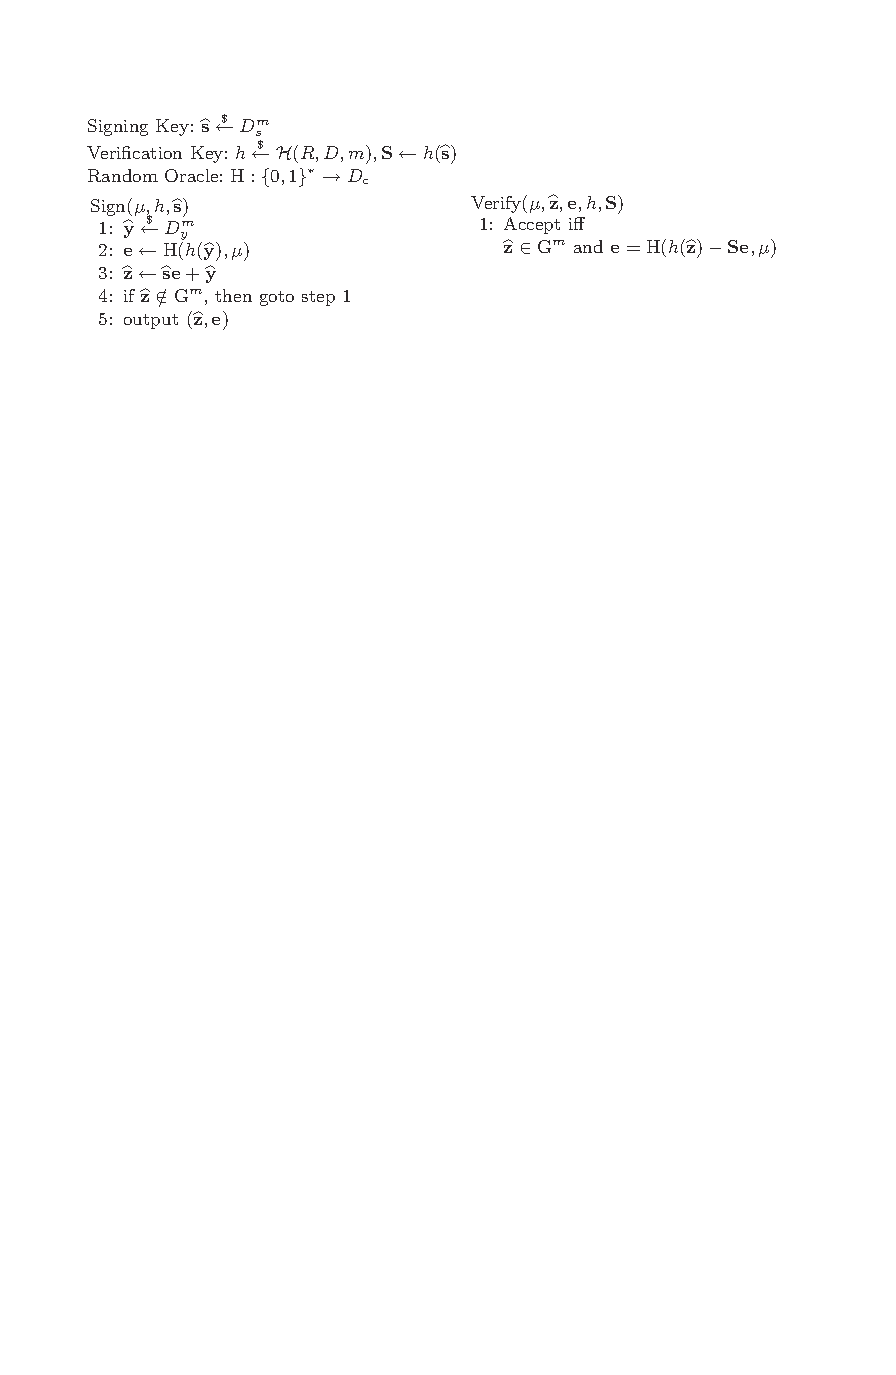
\includegraphics[width=.99\linewidth,trim=40 500 55 54,clip,frame]{plots/loopabortsig}
\caption{The Fiat-Shamir with aborts signature scheme. Figure copied from \cite{fiatshamirabort}[p.~611].}
\label{fig:abortsig}
\end{figure}

\subsection{Fault attacks}
Fault attacks describe a attack model where the attacker is able to choose the physical environment of a device under attack (DUA). The attacker tries to cause the device to malfunction and thus to output the result of a faulty calculation. When the device is running a cryptographic algorithm like an encryption algoritm or signature algorithm a faulty output like a faulty ciphertext or a faulty signature may reveal informytion about the internal state of the device. Thus information of the secret key can be revealed.

The idea of a fault attack was first introduced in \cite{bellcore} which is now infamously called the bellcore attack. The bellcore attack is able to break RSA-CRT with a single faulty signature. DES and AES can be broken with two faulty ciphertexts \cite{fault_survey}. This shows how powerful the fault attack model is.

Faults can be achieved in different ways. In a glitch attack the supply voltage of the DUA is increased or decreased for a short amount if time to a range the device is not rated for, thus causing unexpected, faulty behaviour.
Shining light on the proper place in the right time can also cause a fault. The light can be a simple flash or a precise laser. Because the light needs to be applied directly to the silicone this attack is semi-invasive as the plastic layer has to be removed \cite{older_fault_survey}.
A clock-glitch describes an attack, where the clock signal is disturbed. An attacker could for a single clock cycle significantly reduce the time the clock signal is high. This may result in the processor to skip an instruction. If the skipped instruction would have prevented a loop from aborting, this could be called loop-abort attack.   
Further types of attacks exists, see \cite{fault_survey} for a survey.

For many of the attacks countermeasures do exists and are used in practice. Countermeasures can either be implemented in hardware (e.g. detect high / low voltage) or in software (e.g. check if a previous calculation seems plausible).
 The cat and mouse game between attacker and defenders is still ongoing for the fault attack model.

\subsection{Dilithium}
\label{sec:explaindilith}
Dilithium is currently the only PQC signature scheme recommended and to be standardized by the NIST. \cite{niststatus} The authors proposed parameter sets for the NIST security levels 2, 3 and 5.

The signature works over the ring $\mathcal{R}_q = \mathds{Z}_q[x]/(x^n+1)$ where $q$ is an odd prime. Simplified works as follows:
\begin{itemize}
    \item \textbf{Key generation} First a $k \times l$ matrix $\bm{A}$ of polynomials with uniform coefficients in $\mathds{Z}_q$ is sampled as well as two secret vectors $(\bm{s}_1, \bm{s}_2) \in S_\eta^l \times S_\eta^l$. $S_\eta^k$ and $S_\eta^l$ denote the set of vectors of polynomials with coefficients with absolute value no more than $\eta$ with $k$ or $l$ entries respectively.
    Then the vector $\bm{t} = \bm{A}\bm{s}_1 + \bm{s}_2$ is calculated.
    Finally the public key is the pair $(\bm{A}, \bm{t})$ and the private key is the tuple $(\bm{A}, \bm{t}, \bm{s}_2, \bm{s}_2)$.
    
    \item \textbf{Signature generation}
    First the vector $\bm{y} \in \tilde{S}_{\gamma_1}^l$ is sampled. The only difference between $\tilde{S}_{\gamma_1}^l$ and $S_{\gamma_1}^l$ is that $\tilde{S}_{\gamma_1}^l$ does not contain any polynomial with coefficient $-\gamma_1$.
    Then the high bits of $\bm{w}_1 = \bm{A}\bm{y}$ together with the message $M$ are hashed to the ball $B_\tau$. The Ball $B_\tau$ is the set of polynomials with exactly $\tau$ coefficients being $-1$ or $1$ and the rest zero. The output of the hash function is the commitment value (commitment polynomial) $c$.
    Finally the vector $\bm{z} = \bm{y} + c \bm{s_1}$ is calculated. If the calculated value passes the required tests which ensure that not information about the secrets is leaked, the signature defined as the pair $\sigma = (\bm{z}, c)$ is outputted. Otherwise the process will be repeated until a generated signature passes the tests and can be outputted.
    
    \item \textbf{Verification}
    To verify a signature $\sigma$ of a message $M$ according to a public key \textit{pk} the high bits of $w_1 = \bm{A} \bm{z} - c \bm{t}$ are calculated, we name them $\bm{w}_1'$. Then the signature is verified correctly iff $\norm{\bm{z}}_\infty \leq \gamma_1 - \beta$ and $c = H(M \Vert \bm{w}_1')$.
\end{itemize}
\todo{A: figure of the scheme with all the algs, like vincent maybe?}

To see why the scheme is correct the interesting part is the second condition which is checked. The question is whether following holds:
\begin{align}
\label{dilithium_correct}
	c = H(M \Vert \bm{w}_1') = H(M \Vert \text{HighBits}(\bm{A}\bm{y}))  \overset{?}{=}  H(M \Vert \text{HighBits}(\bm{A} \bm{z} - c \bm{t}))
\end{align}
We know that
\begin{align}
	\bm{A} \bm{z} - c \bm{t} = \bm{A}\bm{y}+c\bm{A}\bm{s}_1 - c\bm{A}\bm{s}_1 - c \bm{s}_2 = \bm{A}\bm{y}- c \bm{s}_2
\end{align}
Per definition of the $c$ and $\bm{s}_2$ the coefficients of  $c \bm{s}_2$ can be at most $β$. Because $β$ is comparatively small this addition / subtraction does not affect the high bits of  $\bm{A}\bm{y}$. Thus the equation \eqref{dilithium_correct} holds and the signature scheme is correct.

The security of the scheme is based on the hardness of the module-LWE problem as well as the SIS problem.

The actual scheme contains many improvements to decrease the memory footprint, decrease execution time and the amount of entropy required but these details are not required for understanding our fault attack nor do they affect our attack.



\subsection{BLISS}
\label{sec:blissdesc}
BLISS \cite{bliss}  is an acronym for \say{Bimodal Lattice Signature Scheme}. It introduced a new more efficient way of rejection sampling by using a bimodal Gaussian distribution instead of the classical Gaussian one.

We will skip some technical parts of the signature scheme and the compression of $\bm{z}_{2}$ as both is not relevant for our attack.

\subsubsection{Key generation}
\label{sec:blisskeygen}
The BLISS public key $\bm{A} \in \mathcal{R}_{2q}^{1 \times 2}$ and private key $\bm{S} \in \mathcal{R}_{2q}^{2 \times 1}$ fulfill that $\bm{A}\bm{S} = q \mod 2q$. The generation is as follows.
First the two polynomials $\bm{f}$ and $\bm{q}$ are sampled with $\lfloor \delta_{1} n \rfloor$ coefficients uniformly from $\{-1, 1\}$ and   $\lfloor \delta_{2} n \rfloor$ coefficients uniformly from $\{-2, 2\}$, rest zero.
The private key $\bm{S}$ is now defined as $\bm{S} = (s_{1}, s_{2})^{t} \leftarrow (\bm{f}, 2\bm{g}+1)^{t}$.
For the public key we first calculate $\bm{a}_{q} = (2 \bm{g} + 1) / \bm{f}$ and set $\bm{A} = (2 \bm{a}_{q}, q - 2) \mod 2q$.

At this point we would like to note that following holds.
\begin{align}
	\bm{a}_{1}\bm{s}_{1} / 2 = ((2\bm{g}+1) / \bm{f})  \bm{s}_{1} =  ((2\bm{g}+1) / \bm{f})  \bm{f} = (2\bm{g}+1) \bm{f}/\bm{f} = 2\bm{g}+1 = \bm{s}_{2}
\end{align}

Thus knowledge of $\bm{s}_{1}$ and the public key suffices to fully recover the secret key. We will use this fact later in our attack.

\subsubsection{Signature generation}
The signature generation begins by sampling two masking polynomials $\bm{y}_{1}$ and $\bm{y}_{2}$ with polynomails from the the discrete Gaussian distribution $D_{\sigma}$.
Then we calculate $u = \zeta \bm{a}_{1} \bm{y}_{1} + \bm{y}_{2} \mod 2q$ and the commitment polynomial $\bm{c} = H({\lfloor \bm{u} \rceil}_{d} \mod p, \mu)$.
Here $H$ is a cryptographically secure hash function mapping to polynomials with exactly $\kappa$ coefficients in $\{-1, 1\}$and the rest zero.
Finally $\bm{z}_{1}$ and $\bm{z}_{2}$ are calculated by first sampling $b \in \{0,1\}$ and then calculating $\bm{z}_{1} \leftarrow \bm{y}_{1} + (-1)^{b} \bm{s}_{1}c$ and $\bm{z}_{2}$ analogously:  $\bm{z}_{2} \leftarrow \bm{y}_{2} + (-1)^{b} \bm{s}_{2}c$.
Now the rejection step and the compression of $\bm{z}_{2}$ is performed. We will leave out the details as they are not relevant for our attack.
Finally the signature is the triple $(\bm{z}_{1}, \bm{z}^{\dagger}_{2}, \bm{c})$ where $\bm{z}^{\dagger}_{2}$ is the compressed version of $\bm{z}_{2}$.

\subsubsection{Signature verification}
% TODO: how does this work ...
This does not make any sense. I do not understand why this signature scheme is correct \ldots
\begin{align}
	\zeta a_{1} z_{1} + \zeta q c &= \zeta a_{1} (y_{1} + (-1)^{b} s_{1}c) + \zeta q c \\
	&=  \zeta a_{1} y_{1} +  \zeta a_{1} (-1)^{b} s_{1}c + \zeta q c \\
	&\overset{\bm{a}_{1} \bm{s}_{1} = \bm{a}_{1} (- \bm{s}_{1})}{=}   \zeta a_{1} y_{1}+  \zeta a_{1} s_{1}c + \zeta q c \\
	&\overset{\bm{a}_{1} \bm{s}_{1} = 1}{=}   \zeta a_{1} y_{1}+  \zeta 1 c + \zeta q c \\
	&=   \zeta a_{1} y_{1}
\end{align}

\subsection{qTESLA}
The qTESLA signature scheme \cite{qtesla} was selected for the second round of the NIST post-quantum cryptography standardization project but was not selected for round three.
When describing the scheme we will leave our various checks which are performed during key generation, signature generation and verification and also some implementation details. The checks include the rejection sampling
but also various checks which aim to counteract fault attacks. None of these checks detect our fault attack because our attack produces perfectly valid signatures. For the reader interested in all details of this signature scheme we refer to \cite{qtesla}.

\subsubsection{Notation}
qTESLA uses two rings, $\mathcal{R}_{q}$ and $\mathcal{R}$ defined as $\mathds{Z}_{q}[x] / <x^{n} + 1>$ and $\mathds{Z}[x] / <x^{n} + 1>$ respectively. The set $\mathcal{R}_{[M]}$ is defined as $\{\sum_{i=0}^{n-1}f_{i}x^{i} \in \mathcal{R} \vert f_{i} \in [-B, B]\}$ and $G$ and $H$ are hash functions. For an add $m$ and $c \in \mathds{Z}$ $c' = c \mod^{\pm} m$ is defined as the unique element $c'$ with $-\lfloor m/2 \rfloor  \leq c' \leq \lfloor m/2 \rfloor$ and $c' = c \mod m$.


\subsubsection{Key generation}
From an initial so called \say{pre-seed}, multiple different seeds like $\textbf{seed}_{y}$ and  $\textbf{seed}_{a}$ are generated to be used to sample the following polynomials.
First the public key polynomials $a_{1}, \ldots, a_{k}$ are sampled from $\mathcal{R}_{q}[x]$ with coefficients uniformly from $\mathds{Z}_{q}$ using $\textbf{seed}_{a}$.
Next the secret polynomial $s$ is sampled from with coefficients distributed following the discrete Gaussian distribution with standard deviation $\sigma$.
The error polynomials $e_{1}, \ldots, e_{k}$ are sample just like $s$ was sampled previously.
The public key polynomials $t_{i}$ are then calculated as $t_{i} = a_{i} s + e_{i}$ for $i \in {1, \ldots, k}$.
Finally the value $g$ is crafted by hashing all public key polynomials $t_{i}$ using $H$.
The secret key is then the tuple $(s, e_{i}, \ldots, e_{k}, \textbf{seed}_{a},  \textbf{seed}_{y}, g)$ and the public key is $(t_{1}, \ldots, t_{k},  \textbf{seed}_{a})$.

\subsubsection{Signature generation}
When signing a message $m$, first a randomness $r$ is collected. Then using this randomness the masking polynomial $y$ is sampled from $\mathcal{R}$ with coefficients in $[-B,B] \cap \mathds{Z}$.
Next the polynomials $v_{i} = a_{i}y \mod^{\pm} q$ are calculated for $i \in \{1, \ldots, k\}$. These polynomials are then hashed together with $G(m)$ and $g$ to construct the commitment polynomial $c$. Finally the $z = y + sc$ is calculated and the signature is defined as the pair $(z, c)$.

\subsection{Signature verification}
Given the public key, private key, a signature $(z, c)$ and the message $m$ to verify a signature we first calculate $w_{i} \leftarrow a_{i} z - t_{i} c \mod^{\pm} q$.
The signature is valid iff both of the following conditions are met:
\begin{itemize}
	\item $z \in \mathcal{R}_{[B-S]}$
	\item $c = H(w_{1}, \ldots, w_{k}, G(m), G(t_{1}, \ldots, t_{k}))$ 
\end{itemize} 

The second condition holds for valid signatures because: \cite[p. 10]{qtesla} % TODO: is this the correct page in the original publush?
% TODO: understand why []_{M} is used then it is not used in the alg? 
\begin{align}
	[a_{i}z-t_{i}c]_{M} = [a_{i}(y+sc) - (a_{i}s+e_{i})c]_{M} = [a_{i}y - e_{i} c]_{M} = [a_{i}y]_{M}
\end{align}
Note that the $[\cdot]_{M}$ operation ignores a certain amount of lower bits of the coefficients of the polynomials.


\section{Lattice based fault attack}
Our attack is inspired by the fault attack of Espitau et al. \cite{espitau} which was described among other schemes against BLISS. They showed a fault during the signing process can reveal the secret key.

\subsection{Attack idea}
The fault they used was a loop-abort fault. In an loop-abort fault a loop is terminated (aborted) prematurely. The loop they targeted was the one sampling the coefficients of the masking polynomial $y_1$. Such a fault would yield a masking polynomial with abnormal low degree. The degree is denoted by $m$. The final signature of BLISS is $(c, z_1 = s_1 c + y_1)$. A faulty signature with a faulty $y_1$ is all the information needed for performing this attack.

The important observation is that if we assume that $c$ is invertable, i.e. $c^{-1}$ exists then the vector $z_1 c^{-1}$ is close to a sublattice of $\mathds{Z}^n$. This assumption that $c^{-1}$ is invertable is true with a high probability. To be more precise we can see that
\[
z_1 c^{-1} - s_1 = c^{-1} y_1 = \sum_{i = 0}^{m-1}y_{1,i}c^{-1}x^i
\]
the sublattice $\mathcal{L}$ is spanned by the vectors $w_i = y_{1,i}c^{-1}x^i$ for $i = 0, \ldots m - 1$ as well as $q\mathds{Z}^n$. The difference of $z_1 c^{-1}$ to that lattice is exactly $s_1$.

Because the dimension of that lattice is still $n$, the secret cannot be recovered directly. But by projecting $z_1 c^{-1}$ as well as the basis vectors of the lattice $\mathcal{L}$ to a subset of its rows, it still holds that the same projection on $z_1 c^{-1}$ is close to the projected lattice and the difference is the projected $s_1$. If the projection is chosen such that the degree is low enough, we can recover a part of $s_1$.  By choosing multiple such projections  we can eventually recover the entire secret polynomial and by that the entire secret key.

It is important to note here that it is crucial that we know which entries of the masking polynomial $y_1$ are faulty. So we need to know in which order the coefficients of $y_1$ are sampled as well as after what iteration the fault occurred. As pointed our in their countermeasures section this attack will not work if this information is not given because e.g. the coefficients are shuffled. In the next section we will describe attack that works efficiently even when this countermeasure is applied.

\subsection{Countermeasures}
\label{sec:countermeasure}
One of the proposed countermeasures by Espitau et al. is to generate the coefficients of the $\bm{y}$ vector in a random order. \cite[p. 13]{espitau} A possible implementation of this can be seen in figure \ref{fig:countermeasure}. It is written in c and uses the \textsc{polyvecl\_uniform\_gamma1} function from the current reference implementation \cite{referenceimpl} which creates the $\bm{y}$ vector is using the on the reference implementation.
The function first samples the coefficients without the shuffling countermeasure and then shuffles them using the Fisher-Yates technique. \cite{fisheryates} The function \textsc{uniform\_random\_interval\_inclusive} generates deterministic pseudo random integers from the set $ \mathds{Z} \cap [0, i]$ using \textsc{seed}, \textsc{nonce} and \textsc{i} as seed. While Espitau et al. need the information about where the faulted coefficients are located, our attack is able to to deal with this lack of information. For the rest of this thesis we will assume that the shuffling countermeasure is implemented just like in figure \ref{fig:countermeasure}.
\begin{figure}
    \centering
    \begin{minted}[breaklines]{c}
        void polyvecl_uniform_gamma1_shuffled(polyvecl *v, const uint8_t seed[CRHBYTES], uint16_t nonce) {
            int32_t tmp;
            uint16_t z;
        
            
            polyvecl_uniform_gamma1(v, seed, nonce);
            
            for (i = N * L - 1; i >= 1; --i) {
                z = uniform_random_interval_inclusive(0, i, seed, nonce);
                tmp = v->vec[i / 256]->coeffs[i % 256];
                v->vec[i / 256]->coeffs[i % 256] = v->vec[z / 256]->coeffs[z % 256];
                v->vec[z / 256]->coeffs[z % 256] = tmp;
            }
        }
    \end{minted}
    \caption{A potential implementation of the shuffling countermeasure.}
    \label{fig:countermeasure}
\end{figure}

Furthermore they propose to add a check after sampling the $y$ vector. The idea is to check whether the $\bm{y}$ vector does not have a too low degree.
They claim that if the signature process is aborted when more than $1/16$'th of the upper coefficients of $\bm{y}$ are zero, the distribution of $\bm{y}$ is skewed so little that it is statistically indistinguishable from the original one and thus the security proof of BLISS still holds. \cite{espitau}[p. 13] In contrast their attack is no longer feasible in this case.


\section{Attacking Fiat-Shamir with aborts based signature schemes}
The attack is based on an integer linear program (ILP) which was originally introduced in the works of  Ulitzsch \cite{ulitzsch} on a Dilithium side channel attack.
In this section we will describe the attacker model and the attack in a general setting. 
We will then later discuss the details to apply this attack to BLISS, Dilithium as well as qTESLA.

\subsection{Preliminaries}
Some text here please % TODO
\subsubsection{Fiat-Shamir with aborts over Rings}
The Fiat-Shamir with aborts signature schemes produce signatures in the form of $z = cs + y$ where $z$ is (part of) the signature (public), $s$ is (part of) the secret key (secret), $c$ is the commitment value (public) and $y$ is the masking vector (secret, (deterministically) random).

The signature schemes we attack work over a Ring $\mathcal{R} = \mathds{Z}_{q}[x] / (x^{n} + 1)$. $q$ and $n$ differ from scheme to scheme and parameter set to parameter set. Though all have in common that $q$ is an odd prime and $n \in \{256, 512, 1024, 2048\}$ is a power of two. Furthermore $z, s$ and $y$ are either elements from $\mathcal{R}$ or from $\mathcal{R}^{l}$ (Dilithium). $c$ is in all cases an element from $\mathcal{R}$. In the following sections we will, for reasons of simplicity, assume that $z, s, y \in \mathcal{R}$. The special case of Dilithium will result in $l$ separate attacks to recover $s \in \mathcal{R}^{l}$, details will be discussed in the Dilithium specific section \ref{sec:attackdilithium}.


\subsubsection{No modular reductions} \label{sec:nomod}
The commitment polynomials are sparse polynomials with coefficients which have small absolute values. While not sparse, the secret polynomials $s$ too have only coefficients with very small absolute value. Thus their product is way below the modulus $q$ even when adding the masking polynomial $y$.  Thus during the signature calculation no modular reductions are applied.

\subsubsection{Linearity}
\label{sec:linearity}
To understand why the partial signature is linear we need to understand how we can describe the multiplication of the commitment polynomial $c$ and the secret polynomial $s$ in the Ring  $\mathcal{R}_q = \mathds{Z}_q[x]/(x^n+1)$  as a linear operation.
We can describe the multiplication as a matrix vector multiplication: A quadratic $n \times n$ matrix $C$, which is the negacyclic matrix of the coefficient vector $c'$ of the commitment polynomial multiplied with the coefficient vector $s'$ of the secret polynomial $s$. Thus $Cs'$ is the coefficient vector of  $cs$ and together with the coefficient vector $y'$ of the masking polynomial $y$ we can write the entire signature as a linear equation system $z' = Cs' + y'$. 

The  linear equation system has two classes of unknowns: The secret coefficients of the secret polynomial $s$, as well as the masking coefficients of the masking polynomial $y$.
We know that a non-negligible amount of masking coefficients are zero. Our attack will thus not bother to recover the values of the masking coefficients, but instead only try to recover the information whether a masking coefficient is zero (most likely because of the fault) or not. Given that we have collected $\sigma$ signatures, we thus have to make $M = \sigma n$ boolean decisions whether a masking coefficient is zero or not. To summarize in our attack we will have to recover the a vector of size $n$ with entries in the range of the secret polynomial coefficients range as well as a boolean vector of size $M$.


\subsection{The attacker model}
\label{sec:attackmodelgeneral}
Here we will assume an attacker which is able create as many different signatures as he likes. He can induce a loop-abort fault in the loop which samples the masking polynomial. When he does so, the faults will cause $1 \leq f \leq n$ zero coefficients in $\bm{y}$ resulting in $m = n - f$ non-zero entries. As afterwards the coefficients are shuffled, he does not know where the zero coefficients are located.

While here we assume that non initialized coefficients are zero, any other constant value would work as well. The attack would need to be adjusted slightly. 
Furthermore the fault can also be of other nature. The attacker could for example target the memory where (part of) the masking vector is stored and set it to zero or another known value. See \cite{espitau}[pp.~153--154] for more details on this.

\subsection{The attack}
Once we have gathered the faulted signatures our attack consists mainly of constructing an instance of Ulitzsch's ILP and solving it. 

\subsubsection{Variables}
\label{sec:ilpvars}
The ILP will use two classes of variables: $n$ variables in the the secret polynomial coefficients range for the secret polynomial $s$. We refer to them as the vector $s'$, just like we did for in the previous sections for the vector containing the coefficients of the polynomial $s$.
Furthermore we will use $M$ boolean variables which describe whether a coefficient of $y$ is zero or not. We will refer to these variables as the vector $x \in \{0, 1\}^M$. For all $i \in {1, \ldots, M}$ $x_{i}$ will be $1$ iff the $(i \mod n)$'th $y$-coefficient of the $\lfloor i / n \rfloor$'th signature is zero. Or in other words: If $Y$ would be a vector containing all coefficients of the all $y$ polynomials obtained by the signatures, simply \say{stacked on one another}, $x_{i}$ will be $1$ iff the coefficient $Y_{i}$ is zero.

\subsubsection{Constraints}
Besides the constraints for the domain of the variables our ILP will have two important additional constraints. Here we choose $K$ to be $\max(\lvert z_{i}' - C_{i}s' \rvert)$.
\begin{align}
	\label{constraint_leq}
	z' - Cs' & \leq K (1 - x) \\
	\label{constraint_geq}
	z' - Cs'  & \geq - K (1 - x)
\end{align}
which can also be written in a more compact way:
\begin{align}
	\label{constraint_compact}
	 - K (1 - x) \leq z' - Cs'  \leq K (1 - x)
\end{align}

To see why these two equations do indeed solve our problem we will will look at two cases: $x_{i} = 0$ and $x_{i} = 1$ for $i \in \{1, \ldots, M\}$.

If $x_{i}$ = 0, the compact constraint \eqref{constraint_compact} will simplify to following.
\begin{alignat}{3}
	 &-K(1 - x_{i}) &&\leq z'_{i} - C_{i}s'  &&\leq K(1 - x_{i}) \\
	 \label{alwaystrue}
	 \Leftrightarrow&- K &&\leq z'_{i} - C_{i}s'  &&\leq K
\end{alignat}

This constraint is always true per our definition of $K$.Thus when the ILP-solver decides on setting $x_{i} = 0$ it decides to ignore equation $i$, i.e. not using its information to recover $s$.

Do note that the ILP-solver can always find a solution that will fulfill all constraints by setting $x = O$, but this solution will not optimize the objective as we will discuss in the next section.  

If $x_{i}$ = 1 and we assume that the ILP-solver finds the correct $s'$, the compact constraint \eqref{constraint_compact} will simplify to following.
\begin{alignat}{3}
	 &-K(1 - x_{i}) &&\leq z'_{i} - C_{i}s'  &&\leq K (1 - x_{i}) \\
	 &-K(1 - 1) &&\leq z'_{i} - C_{i}s'  &&\leq K (1 - 1) \\
	 \Leftrightarrow&0&&\leq z'_{i} - C_{i}s'  &&\leq 0 \\
	 \Leftrightarrow&0 &&\leq  (C_{i}s' + y'_{i}) - C_{i}s'  &&\leq 0 \\
	 \Leftrightarrow&0&&\leq  y'_{i}  &&\leq 0 \\
	  \Leftrightarrow&0&&=  y'_{i}   &&= 0
\end{alignat}
Thus, if the $y'_{i}$ is zero, most likely due to a fault, this constraint will be fulfilled.

Do note that this constraint may also be fulfilled with a choice of $s'$ which is not the secret key we are looking for or even when $y_{i}$ is not zero.
We heuristically assume, supported by our successful simulations, that such events are very unlikely to maximize the objective and will this not be chosen by the ILP-solver.

\subsubsection{Objective}
The ILP will try to maximize the $\sum_{i = 1}^M x_{i}$.
We heuristically assume that this maximum only be reached by choosing $x$ in a way that it's entries are one iff the corresponding to $y$-coefficients are zero, i.e. most likely faulted.
Thus the ILP-solver will distinguish $\bm{z}$ coefficients where the corresponding $\bm{y}$ coefficient is zero from ones where the corresponding $\bm{y}$ coefficients are not zero and solve the set of gathered linear equations at the same time.

\subsection{Pre-filtering equations without faults}
\label{sec:prefilter}
The heavy lifting of classifying whether a coefficient of $\bm{z}$ is zero or not is done by the ILP-solver.
Nevertheless for a certain set of equations we can say with ease that the the corresponding $y$-coefficient can not be zero.
When a coefficient $y_{i}$ is zero we know that $z_{i} = (c s + 0)_{i}$. As we already showed in section \ref{sec:nomod} For all signature schemes we can give a bound $b$ to the absolute value a coefficient of $cs$. Thus if $\lvert z_{i} \rvert \leq b$ holds, we know that $y_{i} \neq 0$ with a probability of $100\%$.

For improved performance we will thus remove any equations where we can tell, by using the aforementioned approach, that their corresponding $y$-coefficient is not zero. We do this before passing these equations to the ILP-solver. In practice this means removing the corresponding entry in the vector $z'$ and the corresponding row in the matrix $C$.

To go even further we can use a lower threshold $t < b$ to pre-filter our equations. Because for every signature scheme we know that the distribution of $cs$ is centered at zero and symmetrical, this will filter out even more equations which are not affected by a fault. On the contrary we will also filter out equation which were indeed affected by the fault. In conclusion we will thus need more signatures to perform our attack. This tradeoff between the amount of signatures required and the false-positive rate of the equations we will be passing to the ILP-solver will be evaluated only for Dilithium in section \ref{sec:evalthreshold}.


With pre-filtering we are able to control the false-positive rate of our equations. Here we classify an equation as being faulted, i.e. $y_{i} = 0$ or not. A true-positive classification would be if we say an equation is faulted and it indeed is. A false-positive classification is when we say an equation is faulted, but it actually is not. Thus the false positive rate is ratio of the number true-positive classifications of our equations to the number of false-positive classifications. This number is an interesting metric for the efficiency of our attack as we will discuss later for Dilithium only.
We are able to control this number by two other parameters:
\begin{enumerate}
	\item the iteration number $m$, after which we induce a fault.
	\item the cutoff value $t$ we use for filtering
\end{enumerate}







\section{Attacking Dilithium}
\label{sec:attackdilithium}

In this section we will discuss the Dilithium signature scheme specific details for our attack.

\subsection{Implementation assumptions and attacker model}
First we assume that a big loop with $nl$ iterations will sample the coefficients for all the coefficients in $\bm{y}$. Secondly we assume that the shuffling occurs throughout all the polynomials of the vector $\bm{y}$. This means that coefficients which where faulted to be zero located in the last polynomial may be shuffled to another polynomial, e.g. the first one.

We thus adjust our attacker model in the way that the attacker will induce a fault after the $1 \leq m \leq nl$ iteration in the loop which samples the coefficients of the masking polynomials.

\subsection{One ILP per polynomial}
The Dilithium signature scheme calculates the signature like follows:
\begin{align}
	\bm{z} = \bm{s}_{1} c + \bm{y}
\end{align}
Where $\bm{z}, \bm{s}_{1}, \bm{y} \in \mathcal{R}^{l}$ and $c \in \mathcal{R}$. We thus can not directly apply the attack mentioned before.
To still use our attack against Dilithium, let $\bm{z}_{i}, {\bm{s}_{1}}_{i}, \bm{y}_{i}$ be the $i$'th polynomial in the respective vector for $1 \leq i \leq l$.
According to definition of $\bm{z}$ it holds for all $1 \leq i \leq l$ that $\bm{z}_{i} = c {\bm{s}_{1}}_{i} + \bm{y}_{i}$. Now, because $\bm{z}_{i}, c, {\bm{s}_{1}}_{i}, \bm{y}_{i} \in \mathcal{R}$ we can apply our attack for every $i$ to recover once secret polynomial of $\bm{s}_{1}$ at a time eventually recover the entire vector $\bm{s}_{1}$.

\subsection{Bound for the difference $z_{i}' - C_{i}s'$ and threshold $t$}
The coefficients of the commitment polynomial $c$ have at most an absolute value of $1$ which can occur at most $\tau$ times. The coefficients of the $\bm{s}_{1}$ polynomials have at most an absolute value of $\eta$. Thus we know that $\lvert  C_{i}s' \rvert \leq \tau \eta = \beta$. Finally the coefficients of the $\bm{y}$ masking polynomials have an absolute value of at most $\gamma_{1}$, thus $\lvert z'_{i} \rvert$ is at most $\tau \eta + \gamma_{1} = \beta + \gamma_{1}$. For the attack on Dilithium we choose $K = 2 \beta + \gamma_{1}$.

To filter equations we will use a threshold of $t = \beta$ as this is the upper bound for coefficients in $\bm{s}_{1}c$ as we just discussed in the previous sections.

\subsection{Creating signatures using only $\bm{s}_{1}$}
As already discussed in section \ref{sec:explaindilith} $\bm{s}_{1}$ is only one part of the secret key. Still $\bm{s}_{1}$ is enough information for an attacker to sign arbitrary messages. Two different methods were presented. One by Bruinderink and Pessel \cite{Groot_Bruinderink_Pessl_2018}[pp.~33--34] and one by Ravi et al. \cite[pp.~12--13]{ravi_2018}. These signatures are indistinguishable from real ones when only given the public key. Only given the secret key we can distinguish the signatures created using only $\bm{s}_{1}$ from the ones created by someone with the entire secret key. 


\section{Attacking qTESLA}
Attacking qTESLA is straight forward because the qTESLA signature scheme strictly follows. Thus we only have to consider the maximum difference $z'_{i} - C_{i}s'$ and the appropriate threshold $t$.

\subsection{Bound for the difference $z_{i}' - C_{i}s'$ and threshold $t$}
\label{sec:qteslathreshold}
The polynomial $s$ has coefficients which follow the discrete gaussian distribution with standard deviation $\sigma$. This distribution being a long-tailed one can thus have theoretically infinitely large samples (coefficients). In practice discrete gaussian samples have a parameter $\tau$ which defines a so called cutoff-value $\tau \sigma$, which limits the samples to be in the domain $[-\tau \sigma, \tau \sigma] \cap \mathds{Z}$. For our evaluation we choose $\tau = 6$ because this is the default one used in SageMath \cite{sagetau}. Thus we can limit the domain of $s$ to be $[-\tau \sigma, \tau \sigma] \cap \mathds{Z}$. This estimation is very conservative and better results may be possible by choosing a smaller $\tau$.

The commitment value $c$ has exactly $h$ non-zero coefficients which are $-1$ or $1$ and the rest is zero. Thus we know that the polynomial $cs$ has coefficients in the range $[-h \tau \sigma, h \tau \sigma]$.

The masking polynomial $y$ has per definition coefficients in the range $[-B, B]$. Thus we can say that the coefficients of $z = y+cs$ are in the interval $[-B h \tau \sigma, B h \tau \sigma] \cap \mathds{Z}$.
Now looking at the difference $z'_{i} - C_{i}s$ we know that that it is bounded by $2 h \tau \sigma + B$. Thus we choose $K = 2 h \tau \sigma + B$.

Consequently we will use $2 h \tau \sigma$ as the threshold $t$.


\section{Attacking BLISS}
The BLISS \cite{bliss} signature scheme was first introduced by Léo Ducas et al. in 2013. With their novel rejection sampling algorithm and other modifications they were able to significantly reduce the standard deviation of their signatures and thus the signature size compared to other post-quantum secure schemes at that time. Their new rejection sampling algorithm is based on the bimodal gaussian distribution. This distribution is obtained in their scheme by choosing a random bit $b \in \{0, 1\}$ and computing a signature vector $z_{1} = s_{1}c + (-1)^{b} y_{1}$. (The entire signature algorithm can be found in section \ref{sec:blissdesc})


\subsection{Special considerations}
Note that the previous two signature schemes do not use such a bit in their signature generation algorithms. To adapt our attack to BLISS we will have to include this bit of information in the ILP.
For a single signature this is just a single bit of information, but as we require more signatures because we fault after more iterations the entropy will grow exponentially and the bits will be harder to recover.
Despite this fact we were able to achieve good results for some of the proposed parameter sets of BLISS.

\subsection{An modified ILP BLISS}
As noted earlier in contrast to the previous two schemes we now have three types of unknowns: The coefficients of the secret key polynomial $s_{1}$, the coefficients of the masking polynomial $y_{1}$ and the bit $b$.  Let $s' \in \{-2, -1, 0, 1, 2\}^{n}$ be the coefficient vector of $s_{1}$, let $x \in \{0, 1\}^{\sigma n}$ the binary / boolean vector which classifies whether a coefficient of one of the $y_{1}$'s is faulted or not just like we described in detail in section \ref{sec:ilpvars}. Finally let $b_{1},  b_{2}, \ldots, b_{\sigma} \in \{-1, 1\}^{\sigma}$ be the variables which describe the sign, which was induced by the bit $b$ ($(-1)^{b}$) for each signature .
Here $\sigma$ denotes the amount of signatures we have acquired and $n=512$ for all BLISS parameter sets proposed by the authors.

Next let the vector $\vec{b} \in \{-1, 1\}^{\sigma n}$ be defined as
\begin{align}
	b = (\overbrace{b_{1}, b_{1}, \ldots, b_{1}}^{n \text{ times}}, \overbrace{b_{2}, b_{2}, \ldots, b_{2}}^{n \text{ times}}, \ldots, \overbrace{b_{σ}, b_{σ}, \ldots, b_{σ}}^{n \text{ times}})^{T}
\end{align}

Finally we can redefine the two constraints \eqref{constraint_leq} and \eqref{constraint_geq} of the ILP as follows. Do note that additional constraints do define the domain of the different variables are required.
\begin{align}
	\label{constraint_leq_bliss}
	z' - \vec{b} \cdot Cs' & \leq K (1 - x) \\
	\label{constraint_geq_bliss}
	z' - \vec{b} \cdot Cs'  & \geq - K (1 - x)
\end{align}
The symbol $\cdot$ (dot) between $\vec{b}$ and $Cs$ is defined here as the coefficient-wise multiplication of the two vectors.

\subsection{Bound for the difference $z_{i}' - C_{i}s'$ and threshold $t$}
Let $d_{1} = \lfloor nδ_{1} \rfloor$ and $d_{2} =  \lfloor nδ_{2} \rfloor$. For all by the authors proposed parameter sets $C_{i}s'$ has at most an absolute value of $2 d_{2} + κ - d_{2}$. Thus we will use $2 * d_{2} + κ - d_{2}$ as the threshold.
The coefficients of $y_{1}$ follow the discrete gaussian distribution with a standard deviation $σ$. As already discussed in detail in section \ref{sec:qteslathreshold} we can limit the absolute values of the coefficients of $y_{1}$ to $τ σ$ with $τ = 6$. Thus we know that $\lvert z_{i}' \rvert \leq 2 d_{2} + κ - d_{2} + τ σ$. Thus we choose $K = 2 (2 d_{2} + κ - d_{2}) + τ σ$.


\subsection{Recovering the entire secret key}
This attack will only recover the secret polynomial $s_{1}$ but not the second secret polynomial $s_{2}$. This is not a problem as $s_{1}$ is sufficient to recover the entire secret key as we noted in detail in section \ref{sec:blisskeygen}.















\section{Simulations: theory}
In this section we will discuss on what assumptions we base our simulations and what kind of parameters we will evaluate. 
\subsection{Assumptions}
\label{sec:simassumptions}
We assume an attacker as described in section \ref{sec:attackmodelgeneral}.
Further will always assume that we as the attacker will have at least as much information as would be sufficient to break the signature scheme if the shuffling countermeasure would not be used. This translates to the fact that we will always have $n$ or more faulted coefficients per secret polynomial which correspond to at least $n$ linear independent equations. This is because without the shuffling countermeasure an attacker would know which coefficients were faulted (the last few), take the corresponding linear equations and solve them using gaussian elimination.

\subsection{Notion of success}
\label{sec:simsuccess}
For a certain $m$ we will say that we were successful in breaking the signature scheme, if we manage to succeed recovering the entire secret in at least 2 two out of three tries, i.e. we have a success rate of at least around $66\%$. Each try fails after a timeout of 5 minutes wall time.

\subsection{Parameter evaluation}
When we use only the minimal mount of signatures required to fulfill our aforementioned requirements the attack will not show optimal results.
Thus, for Dilithium, we will evaluate two parameters of our attack which we hope to improve our results:
\begin{enumerate}
	\item surplus of equations $p$
	\item threshold $t$
\end{enumerate}
For qTESLA and BLISS we will only evaluate the parameter $p$. 

The surplus of equations $p$ is the minimal amount of additional faulted equations (relative to the minimum described in  \ref{sec:simsuccess}).
In our simulations we control this value by generating signatures until we can guarantee that the secret polynomial(s) has at least $n + p$ faulted equations out of which where exist $n$ linear independent ones.

The threshold parameter is used as a metaphor for false-positive rate as described in detail in section \ref{sec:prefilter}. The lower the threshold, the lower the false-positive rate and vice versa.
The false-positive rate is dependent on both, $m$ and $t$. Thus for a fixed $m$ the false-positive rate only depends on $t$.

We choose the two parameters based on the following two arguments.

We argue that a greater surplus of equations opens more choices to the ILP-solver to classify enough equations properly and thus the searchspace will more likely contain an easy-to-find path to a solution.
The arguing with the false-positive rate is that a lower false-positive rate makes (random) positive classification guesses of the ILP-solver more likely to be correct and thus the ILP-solver should reach its objective quicker, eventually recovering the secret polynomial.


When we perform an attack with default parameters, we mean we will use a threshold which does not filter any true-positive equations, we fulfill the assumptions in section \ref{sec:simsuccess} and all that with the minimal amount of signatures required.

\subsection{Parameter evaluation strategy}
In general the simulations aim to find out how lax we can be in the timing of the fault, which translate to how high we can go with the iteration number $m$, after which we will induce a fault. While in the simulations we will fault exactly $f$ coefficients per signature, the simlation results can be translated to an attacker who faults on average $f$ coefficients per signature.

The parameters $p$ and $t$ will be evaluated as follows:
Let $m'$ be highest iteration number we were able to succeed with default parameters.
We will start at $m = m' + 1$ as we know of that our attack will succeed for $m'$.
We will then step by step increase $m$ and simulate whether we still succeed. If we do not succeed, we will simulate the attack again, but this time we will increase or decrease the parameter value we are evaluation depending on what action will help the attack to succeed.
Using this strategy we will be able to determine for every $m$ if our attack succeeds, and if yes, what parameter value is necessary for success.


\section{Simulation results}
In this section we will discuss the results of our simulations. After we describe the hard- and software used for our simulations we will start with thorough discussion on the results for Dilithium, as we will evaluate and compare both the parameters $s$ and $p$. Next we will follow with qTesla as well as BLISS.

\subsection{Simulation hard- and software}
\label{sec:practise_server}
The ILP-solver used for our simulations is Gurobi \footnote{\url{https://www.gurobi.com/}}.
Our simulation is written in Python using the Numpy library \footnote{\url{https://numpy.org/}} and the gurobipy library \footnote{\url{https://pypi.org/project/gurobipy/}} for the Gurobi Python bindings. All simulations were run on a computer with a Intel\textsuperscript{\textregistered} Xeon\textsuperscript{\textregistered} Processor E7-4870 (4 sockets, 10 cores, using 40 threads in total @ 2.4GHz) with 500GB of RAM.

\subsection{Dilithium}
For Dilithium we will first discuss the results when the default / minimal parameters are used. Then we will discuss the results for both, the parameter $p$ and the parameter $t$. Finally we will compare the results of both parameters.

\subsubsection{Default parameters}
\label{sec:min_sig_amount}

\begin{figure}
	\centering
	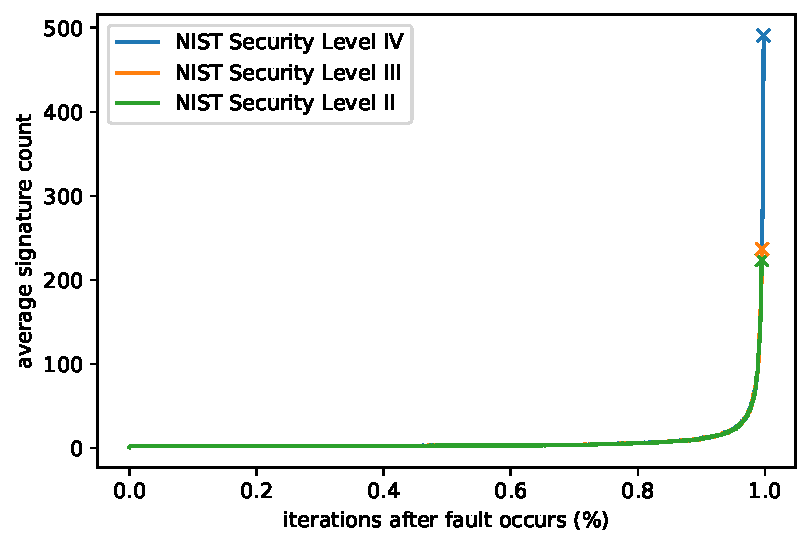
\includegraphics[width=\linewidth]{plots/dilithium_sigcount_noparams}
	\caption{Average amount of signature required for a successful attack per iteration after fault occurs in percent. The amount of signatures is very similar throughout all security levels for early iteration aborts. Thus the green line covers the other two. Crosses indicate the maximum signature count.}
	\label{fig:dilithiumsigcountnoparams}
\end{figure} 

When using the default threshold described in section \ref{sec:prefilter} and a surplus of $0$ our attack succeeds for $f$ as low as $5$, $6$ and $4$ requiring $224$, $236.5$ and $491$ signatures on average for the NIST security levels $2$, $3$ and $5$ respectively.
Further we observe that the higher the NIST security level the more signatures are required. This is due to the fact that minimum amount of equations increases as the security level increases  because the parameter $l$ increases for every security level.  Recall that the minimum amount of required equations is $nl$. The amount of signatures required per $m$ is depicted in figure \ref{fig:dilithiumsigcountnoparams}.

\subsubsection{Surplus of equations}
\label{sec:dilithiumsurplus}

\begin{figure}%
	\centering%
	\begin{subfigure}{.5\textwidth}%
		\centering%
		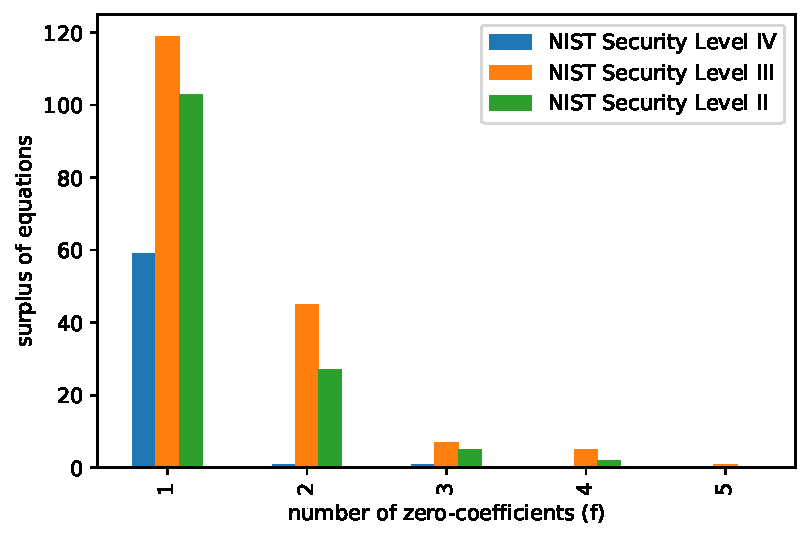
\includegraphics[width=.95\linewidth]{plots/dilithium_surplus}%
		\caption{Surplus of equations per $f$}%
		\label{fig:dilithiumsurplus}%
	\end{subfigure}%
	\begin{subfigure}{.5\textwidth}%
		\centering%
		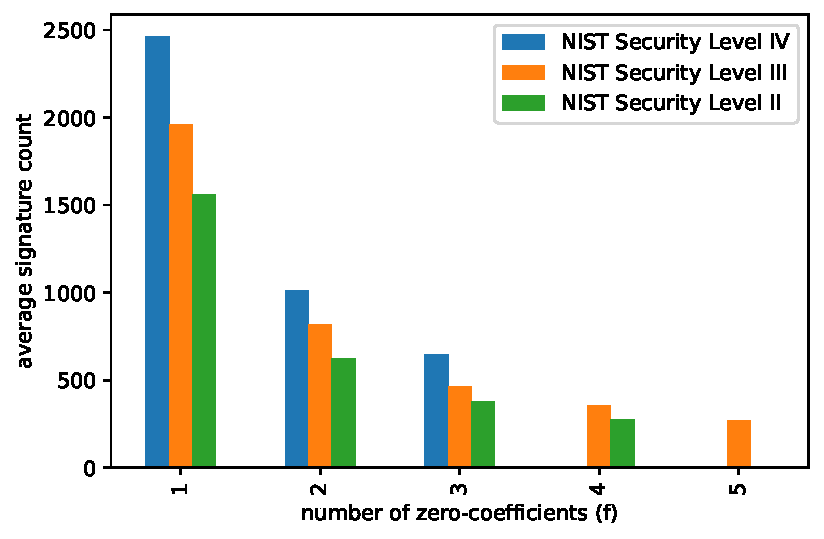
\includegraphics[width=.95\linewidth]{plots/dilithium_sigcount_upper}%
		\caption{Corresponding signature count per $f$.}%
		\label{fig:dilithiumsigcountsurplus}%
	\end{subfigure}%
%
	\caption{The minimal required surplus of equations and the corresponding signature count per $f$. If a bar is not present it means that no surplus was required for that security level and $f$.}
	\label{fig:dilithiumsigcountsurplus}%
\end{figure}

Our simulation results show, that for every $m$, we are able to succeed our attack.
This means that an attacker who is able to (on average) fault a single coefficient of $\bm{y}$ he can recover $\bm{s}_{1}$, given that he can do it on around $1562$,  $1959.5$, $2465.0$ signatures for NIST security level $2$, $3$ and $5$ respectively. The surplus of equations required per $m$ as well as the amount of signatures required per $m$ are depicted in figure \ref{fig:dilithiumsigcountsurplus}.



\subsubsection{Threshold}
\label{sec:evalthreshold}

\begin{figure}%
	\centering%
	\begin{subfigure}{.5\textwidth}%
		\centering%
		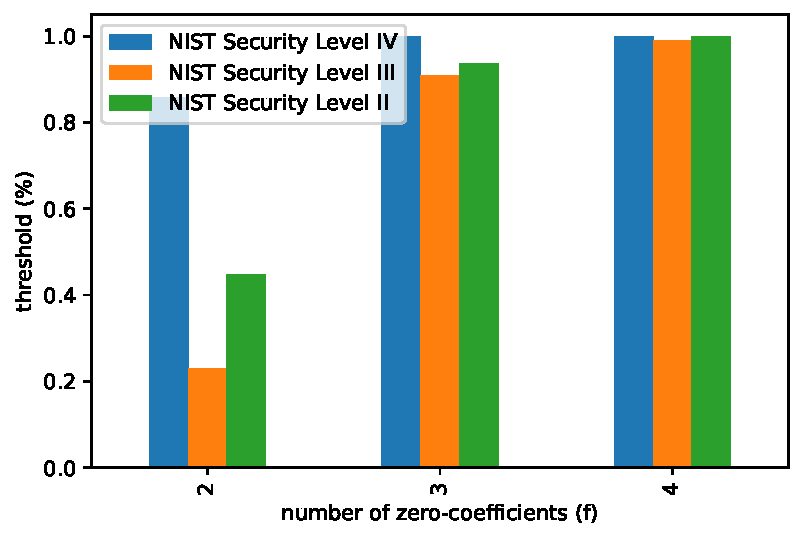
\includegraphics[width=.95\linewidth]{plots/dilithium_threshold_percent}%
		\caption{Maximum possible threshold ($\%$).}%
		\label{fig:dilithiumthreshold}%
	\end{subfigure}%
	\begin{subfigure}{.5\textwidth}%
		\centering%
		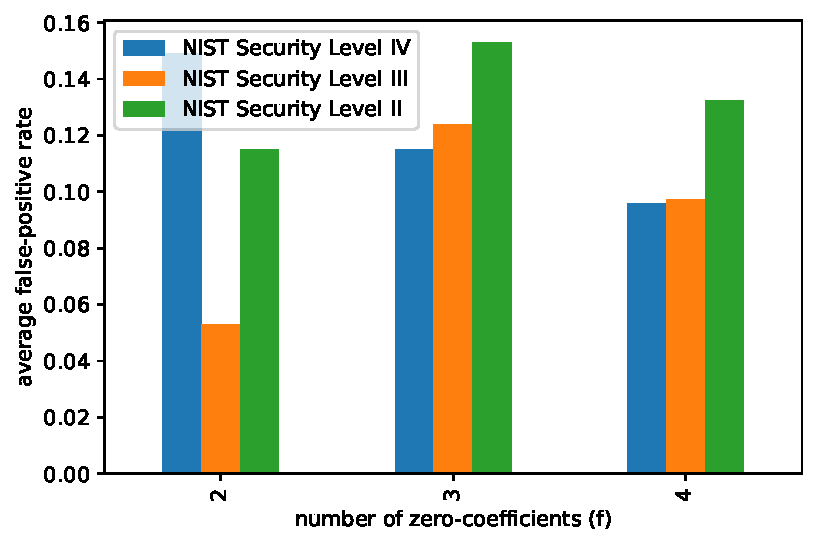
\includegraphics[width=.95\linewidth]{plots/dilithium_threshold_fpr}%
		\caption{Corresponding false-positive rate.\phantom{}}%
		\label{fig:dilithiumthresholdfpr}%
	\end{subfigure}\\\vspace{1em}%
	\begin{subfigure}{.5\textwidth}%
		\centering%
		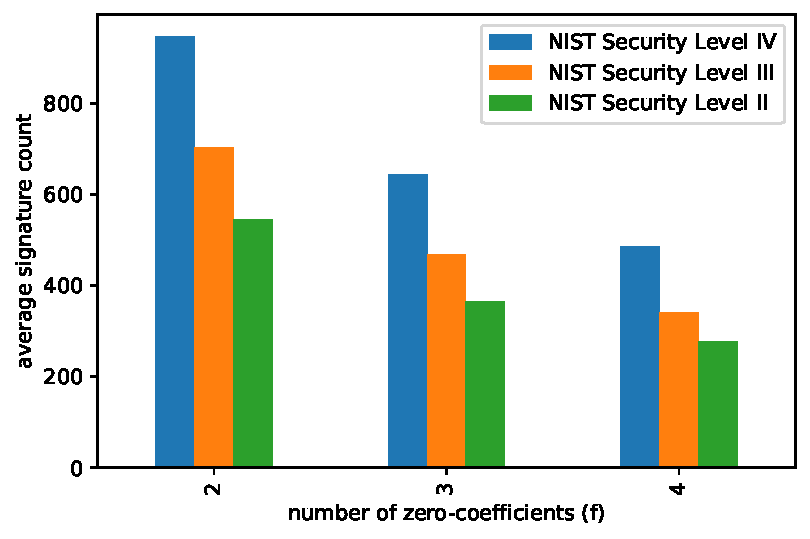
\includegraphics[width=.95\linewidth]{plots/dilithium_threshold_sigcount}%
		\caption{Corresponding signature count.}%
		\label{fig:dilithiumthresholdsigcount}%
	\end{subfigure}%
%
	\caption{The maximum possible threshold per $f$ and the corresponding false-positive rate as well as the corresponding signature count.}
	\label{fig:dilithiumthresholdall}%
\end{figure}
We evaluated the threshold parameter for $f \leq 4$ as for higher $f$ our attack succeeded without needing the additional threshold parameter.
We were able to succeed our attack for all $f \leq 2$ for all NIST security levels. We were not able to succeed our attack for any security level when only a single coefficient is faulted.

In figure \ref{fig:dilithiumthreshold} we observe that as $f$ decreases ($m$ increases) we require a lower threshold to succeed. This can be explained because as $f$ decreases for a fixed threshold we will have an increased false-positive rate. To achieve the same false-positive rate as we had with $f + 1$ we require a lower threshold. 

If we compare the  threshold for fixed $f$ but different security levels we notice that the relative thresholds are similar for $f = 3, 4$, but very different for $f = 2$. Latter we can not properly explain. It might be due to lucky/unlucky ILP instances.

Inspecting the false-positive rate in figure \ref{fig:dilithiumthresholdfpr} for $f=3, 4$ we observe that the higher the security level the lower the false-positive rate. This behavior is expected as $l$ ILPs to be solved per attack and $l$ increases as the security level increases. As all security levels have the same time limitation, higher security levels need to solve more ILPs per fixed time and thus have less time per ILP. To solve an ILP in a shorter timeframe the attacker requires easier ILP instances. Thus a lower false-positive rate is required. Finally again we can not properly explain the data for $f=1$.

The signature count (figure \ref{fig:dilithiumthresholdsigcount}) increases as $f$ decreases and also for a fixed $f$ the signature count increases as the security level does.
Both of these phenomena have been explain in the previous section \ref{sec:dilithiumsurplus}.

\subsubsection{Comparison}
\label{sec:dilithiumcompare}
Looking at the aspect of for which $m$ we are able to perform a successful attack we can see that when using the \say{surplus of equations} parameter we can do so for any $m$, whereas using the \say{threshold} parameter we are only able to do so for for all $m \leq 1278$. 
When comparing the amount of signatures which are needed for a successful attack per $m$ we  observe that when using the \say{surplus of equations} parameter we need slightly more signatures to succeed than with \say{threshold}.

We value the fact that we are able to succeed with a higher $m$ more than the slightly decreased signature amount. Thus we conclude that the parameter \say{surplus of equations} has a slightly bigger impact on the attack performance than \say{threshold}.
Albeit we note that both parameters have impact on the attack performance. While the optimal solution is probably to use both parameters together with a certain weight, the attack results of the \say{surplus of equations} parameter are good enough for our use-case so that we will not do further research to increase the performance.
Furthermore we believe that these results will be similar for the other two signature schemes. Thus we will only evaluate the \say{notion of success} parameter for the other signature schemes.

\subsection{qTESLA simulation results}
\label{fig:resqtesla}

\begin{figure}[p]
\centering
\begin{subfigure}{.5\textwidth}
  \centering
  
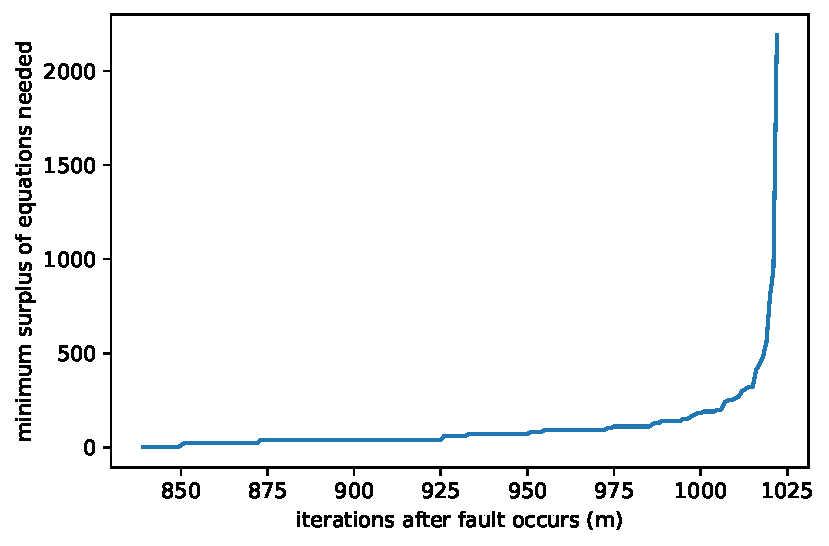
\includegraphics[width=.9\linewidth]{plots/server_qtesla_i_surplus}%
  \caption{minimum required surplus}
  \label{fig:resqteslasurplus}
\end{subfigure}%
\begin{subfigure}{.5\textwidth}
  \centering
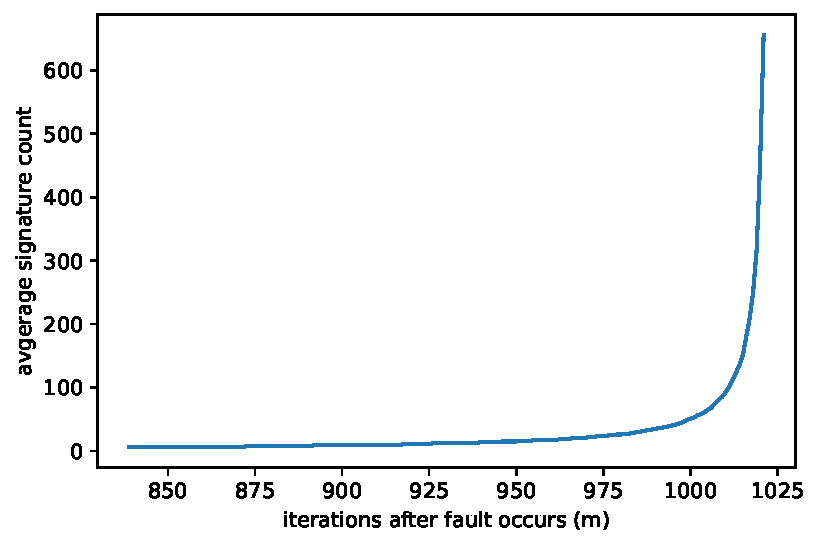
\includegraphics[width=.9\linewidth]{plots/server_qtesla_i_sigcount_surplus}%
  \caption{average amount of faulted signatures}
  \label{fig:resqteslasigs}
\end{subfigure}

\caption{qTESLA simulation results. An attacker can break the shuffling countermeasure if he can at least (on average) cause two faulted entries in $y$ per signature.}
\end{figure}


The simulation for qTESLA were performed using the same soft- and hardware described in section \ref{sec:practise_server}.
With using only the minimal amount of signatures the attack succeeds for all $m \leq 849$.

When evaluating the parameter we choose to increase it by 10 whenever the attack fails. We do this because in depending on the parameter set qTESLA's $n$ is 4 or 8 times as large as in Dilithium's and thus the increase of the parameter relative to $n$ is smaller. To finish our simulations in a reasonable amount of time we therefore increase the step size.

Our simulation results show that we are able to break the shuffling countermeasure for the parameter set \texttt{qTESLA-p-I} (NIST security category 1) but not so for the parameter set  \texttt{qTESLA-p-I}  (NIST security category 3) for any reasonable $m$.
The exact results for parameter set  \texttt{qTESLA-p-I}  can be found in figure \ref{fig:resqtesla}.
 
Compared to Dilithium and BLISS qTesla works on a way higher dimension even in the NIST security category I ($n = 1024$). Thus we assume this is the reason we were unable to break NIST security category III of qTESLA, as it doubles the dimension compared to security category I to $n = 2048$. Higher dimensions result in higher variable-count in the corresponding ILP, exponentially increasing the difficulty to solve it.

\subsection{BLISS simulation results}
With using only the minimal amount of signatures the attack succeeds for all $m \leq 235$. Using the \say{surplus of equations} parameter we are able to succeed our attack for until $m = 367$ using 5 faulted signatures.




\section{Conclusion and Countermeasures}
In this thesis we showed the shuffling countermeasure can be efficiently broken by using ILPs. With the appropriate amount of signatures we were able to break the Dilithium, qTESLA and BLISS signature scheme when $1$ or $2$ or $???$ 

\subsection{Countermeasures}
Bindel et al. \cite{sensitivity}[p.~74] presented a countermeasure against an attack, which skipped the addition of the entire masking polynomial $y$: Instead of adding the error polynomial on to the $sc$ vector, we add the $sc$ and $y$ into a new variable. This does not directly apply to our attack scenario as we do not cause $y$ to be zero by skipping its addition but instead we skip only part of its addition by skipping iterations in the sampling loop. Still, we can use this idea as a countermeasure against our attack by combining the sampling of $y$ and the addition of $y$ and $sc$ into a single loop, instead of doing both operations separately. Thus if we try to abort the loop which samples $y$, we also abort the addition of $sc$ and $y$. Thus for all coefficients we fault, we only get unininitized memory which does not contain any information.

As a possible countermeasure to protect BLISS, and possible other signature schemes which use the discrete gaussian distribution for their masking vectors, blinded gaussian shuffling can be used. This countermeasure was first introduced by Saarinen \cite{multishuffle}[p.~82] to counteract side-channel attacks against discrete gaussian sampler. The general idea is that then adding two discrete gaussian distributed random variables $X$ and $Y$ with a standard deviation of $\sigma$, centered at zero, $X + Y$ is also follows the discrete gaussian distribution, centered at zero with a standard deviation of $\sqrt{σ^{2} + σ^{2}}$. We can use this fact to construct a $y$-vector with standard deviation $σ$ by adding $k$ discrete gaussian distributed vectors with standard deviation $σ' = \frac{σ}{\sqrt{m}}$. Furthermore we shuffle all vectors before we add them together. This would require an attacker to perform $k$ loop-abort faults and still the expected amount of zero coefficients in the resulting masking vector would be exponentially small in $k$. Latter because, a faulted-coefficient of a sampled polynomial might be added with a non-faulted coefficient the other vector due to the shuffling. Additionally this also protects against side-channel attacks. On the other hand this strategy also decreases the performance of the discrete gaussian sampler by $k$-fold. 


\section{Future work}
While we believe that our simulations already stress the need for more countermeasure research it would be interesting to see this attack to be implemented in practice on real hardware to further proof the point. Furthermore it might be possible to improve the performance of the attack by combining the $p$- and $t$-parameter in an optimal fashion.

\printbibliography

\end{document}

